\chapter{Resultados Preeliminares}
\section{Estudo de Caso}
O LAPPIS possui uma infraestrutura de servidores que vinha possibilitando a disponibilização de serviços e ferramentas de utilidades para FGA. Destaca-se as ferramentas Redmine e Dotproject, utilizadas nas disciplinas de metodologia de desenvolvimento de software e Gestão de Portiflólio e Produto, bem como possibilitava a disponibilização de máquinas virtuais utilizadas como ambientes de testes para desenvolvimento do Portal do Software Público, e para sistemas que estavam sendo desenvolvidos também pelo  lappis, tais como o SRA(sistema de registro de atendimento) e o SGD(sistema de gestão de desempenho). Entretanto tais recursos físicos vinham sendo subutilizados, devido aos seguintes fatores.
\begin{itemize}
 \item Versão do hypervisor desatualizada.
 \item Ausência de uma interface de gestão para máquinas virtuais.
 \item centralização do conhecimento.
\end{itemize}
      
      O hypervisor utilizado para disponibilização máquinas virtuais era o XEN na versão 4.1. Desse modo, com  o hypervisor nessa versão era impossível a disponibilização de máquinas virtuais com a versão de sistemas operacionais mais recentes tais como \textit{Debian 7}, \textit{Debian 8} e \textit{Centos 7}. O que tornava difícil também, a tarefa de disponibilizar ambientes de testes com sistemas operacionais atualizados, para sistemas em desenvolvimento pelo LAPPIS. A falta de uma interface de gerenciamento dificultava atividades triviais tais como instanciação, criação de imagens e migração de máquinas virtuais bem como visibilidade de uso de recursos. Por fim, a centralização do conhecimento impactava uma dependência problemática do profissional responsável pela implementação dessa infraestrutura. Assim, na sua ausência a equipe por parte do lappis responsável por essa infraestrutura, encontrou sérias dificuldades em manter a disponibilização de ambientes virtuais. Essa baixa visibilidade dos procedimentos adotados na infraestrutura, também promovia insegurança por parte da equipe em arriscar no desenvolvimento de mudanças relacionadas à essa infraestrutura. Dessa modo, o uso de recursos de harwdare disponíveis para provimento de serviços úteis tanto para o LAPPIS quanto para a FGA estava comprometida. 
      
      Apartir disso, dado a inviabilidade de continuar com essa infrestrutura, chegou-se a conclusão que o melhor caminho a ser adotado era a reformulação da mesma.Desse modo,adotou-se os seguintes procedimentos:
\begin{itemize}
      \item Migração de máquinas virtuais para um dos servidores, de modo que o outro permanecesse liberado para a implementação inicial de uma plataforma em nuvem.
      \item	Implementação de uma plataforma em nuvem que atendessem as necessidades do LAPPIS no servidor físico.
      \item Consolidação de toda infraestrutura física sob as novas soluções de nuvem.
\end{itemize}      
      
      
Desse modo, com os próprios colaboradores do LAPPIS desenvolvendo esse tipo de inciativa, a expectativa era que o problema relacionado com a centralização do conhecimento fosse sanado. A implementação de uma solução de nuvem, e consequetemente, uso de outro hypervisor ou até mesmo o próprio XEN atualizado proporcionaria a solução dos problemas relacionados a falta de gerenciabilidade e a disponibilização de máquinas virtuais com sistemas operacionais atualizados, respectivamente.        
                
\section{Infraestrutura}
A infraestrutura basicamente é composta de três servidores físicos e de máquinas virtuais que compartilham o uso de recursos desses servidores. Dois desses possuem a mesmas configurações: 
\begin{itemize}
	\item Servidor em \textit{rack} \textit{Dell PowerEdge r620.}
	\item 24 processadores \textit{Intel Xeon }, 2.0GHz.
	\item 64 GB de Memória DDR3.
	\item 2TB SATA HDD.
	\item 4 interfaces \textit{EThernet 10/100/1000-BaseT.}
\end{itemize}
Esses servidores são identificados como \textit{Solarian} e \textit{Imperius} e estavam sendo utilizados como os provedores de máquinas virtuais.O terceiro servidor físico possui a seguinte configuração:
\begin{itemize}
	\item Servidor dell em torre.
	\item 8 processadores \textit{Intel Xeon }, 3.2GHz.
	\item 24 GB de Memória DDR3.
	\item 2TB SATA HDD.
	\item 1 interface \textit{EThernet 10/100/1000-BaseT.}
\end{itemize} 
Esse servidor é identificado como \textit{Polaris} e seu uso se limitava a uma estação de trabalho convencional. A imagem a seguir apresenta um esquema onde mostra a alocação das máquinas virtuais nos servidores, em seguida é feita uma breve descrição dos serviços oferecidos.

\section{Migração de Máquinas Virtuais}
Para implementação de uma solução de plataforma em nuvem, os procedimentos adotados consistiam em usar inicialmente um dos servidores como ambiente físico  para testes iniciais da plataforma em nuvem. Assim que a mesma estivesse estabilizada, o outro servidor seria agregado a essa solução. Desse modo, uma maneira encontrada para que esses procedimentos fosse feitos sem ter a indisponibilização dos serviços por um grande período de tempo foi a migração de todos os serviços para um único servidor. Assim, teria-se um servidor livre para uma implementação e investigação incial dessa plataforma em nuvem, enquanto que o outro servidor estaria disponibilizando os serviços em uso. Com isso, o servidor escolhido para essa implementação e investigação inicial da plataforma em nuvem foi o \textit{solarian}. 

Dado que as máquinas virtuais utilizavam discos \textit{LVM}, o procedimento adotado foi:
\begin{itemize}
  \item Criação de imagens das máquinas virtuais com auxílio  \textit{LVM} e do comando \textit{dd}.
  \item Transferência dessas imagens para o servidor \textit{Imperius}.
  \item Restauração dessas imagens em discos \textit{LVM} no servidor \textit{Imperius}
  \item Criação de máquinas virtuais no servidor \textit{Imperius} utilizando as imagens restauradas em discos LVM.
  
\end{itemize}

Assim, todas as máquinas virtuais que estavam no servidor \textit{Solarian} foram transferidas para o servidor \textit{Imperius}, possibilitando assim que fosse iniciado a implementação da plataforma em nuvem em um servidor físico.


\section{Implementação da Plataforma em nuvem}
Para implementação da plataforma em nuvem duas ferramentas foram previamente abordadas \textit{Cloudstack} e \textit{Opennebula}. O \textit{Cloudstack} é uma ferramenta código aberto projetada para implantar e gerenciar uma ampla rede de máquinas virtuais, possibilitando a implantação de uma infraestrutura como serviço de alta disponibilidade \cite{cloudstack}. Em um modelo simplificado, o cloudstack é composto de uma máquina de gerenciamento e dos recursos a serem gerenciados. Tais recursos compreende: faixa de endereços \textit{IP}, dispositivos \textit{storage},servidores e \textit{VLAN'S}. Para implementação em uma configuração mínima, pode se utilizar uma máquina dedicada apenas para a interface de gerenciamento, mantendo o servidor físico apenas com o hipervisor, ou utilizar o servidor físico executando a interface de gerenciamento e o hipervisor simultaneamente. 

\begin{figure}[!htb]
\centering
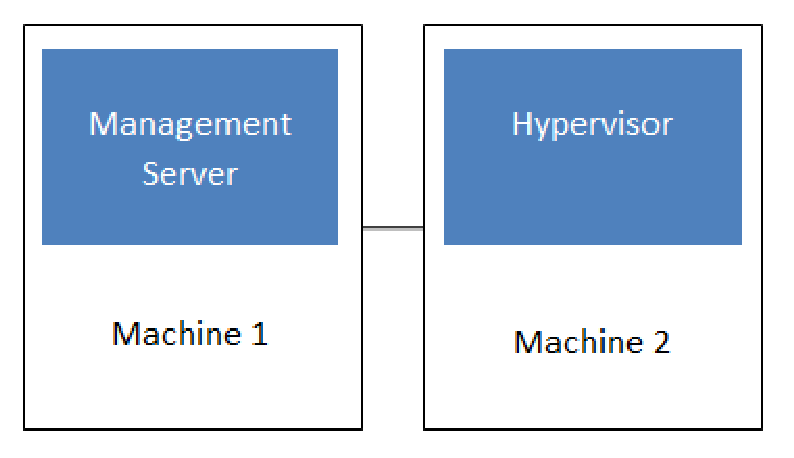
\includegraphics [keepaspectratio=true,scale=0.60]{figuras/cloudstack_minimal.eps}
\caption{Visão simplificada de uma instalação mínima do cloudstack}
\cite{cloudstack}.
\label{cloudstatck_minimal}
\end{figure}

Em modelo mais complexo, o cloudstack apresenta seu pontencial de disponibilidade escalabilidade e gerenciamento. Proporcionando uma modelagem de várias
infraestrutura em nuvens em uma determinada região. Desse modo o cloudstack possui os seguintes níveis de abstrações \cite{shape}:

\begin{itemize}
\item \textbf{Regiões:} são a primeira e maior unidade de escala de uma implementação de uma cloud com CloudStack. Uma Região consiste em multiplas Zonas de Disponibilidade, a segunda maior unidade de escala.
\item \textbf{Zonas: } Tipicamente existe apenas uma Zona por Data Center e cada Zona contem PODs, Hosts e Storage.
\item \textbf{Pods: } PODs tem propriedades lógicas e físicas com componentes como endereçamento IP e algoritmo de alocação de Máquinas Virutais sendo influenciados por PODs dentro de uma Zona.
\item \textbf{Clusters: } São simples grupos de servidores homogêneos combinados com um Storage Primário. Cada Cluster utiliza um mesmo tipo de hypervisor mas em uma Zona pode ceoxistir combinações de todos os hypervisores suportados. Cada Cluster utiliza um mesmo tipo de hypervisor mas em uma Zona pode ceoxistir combinações de todos os hypervisores suportados.
\item \textbf{Hosts: } Responsável por disponibilizar a camada de computação real em que Máquinas Virtuais são executadas.
\item \textbf{Storage Primário: }  onde os discos das Máquinas Virtuais residem e pode ser utilizado o disco local de um Host ou um storage compartilhado como NFS, iSCSI, Fiber Channel, etc.
\item \textbf{Storage Secundário:} onde é armazenado os Templates de Máquinas Virtuais, arquivos ISO e Snapshots e é utilizado o protocolo NFS para este Storage
\end{itemize}


\begin{figure}[!htb]
\centering
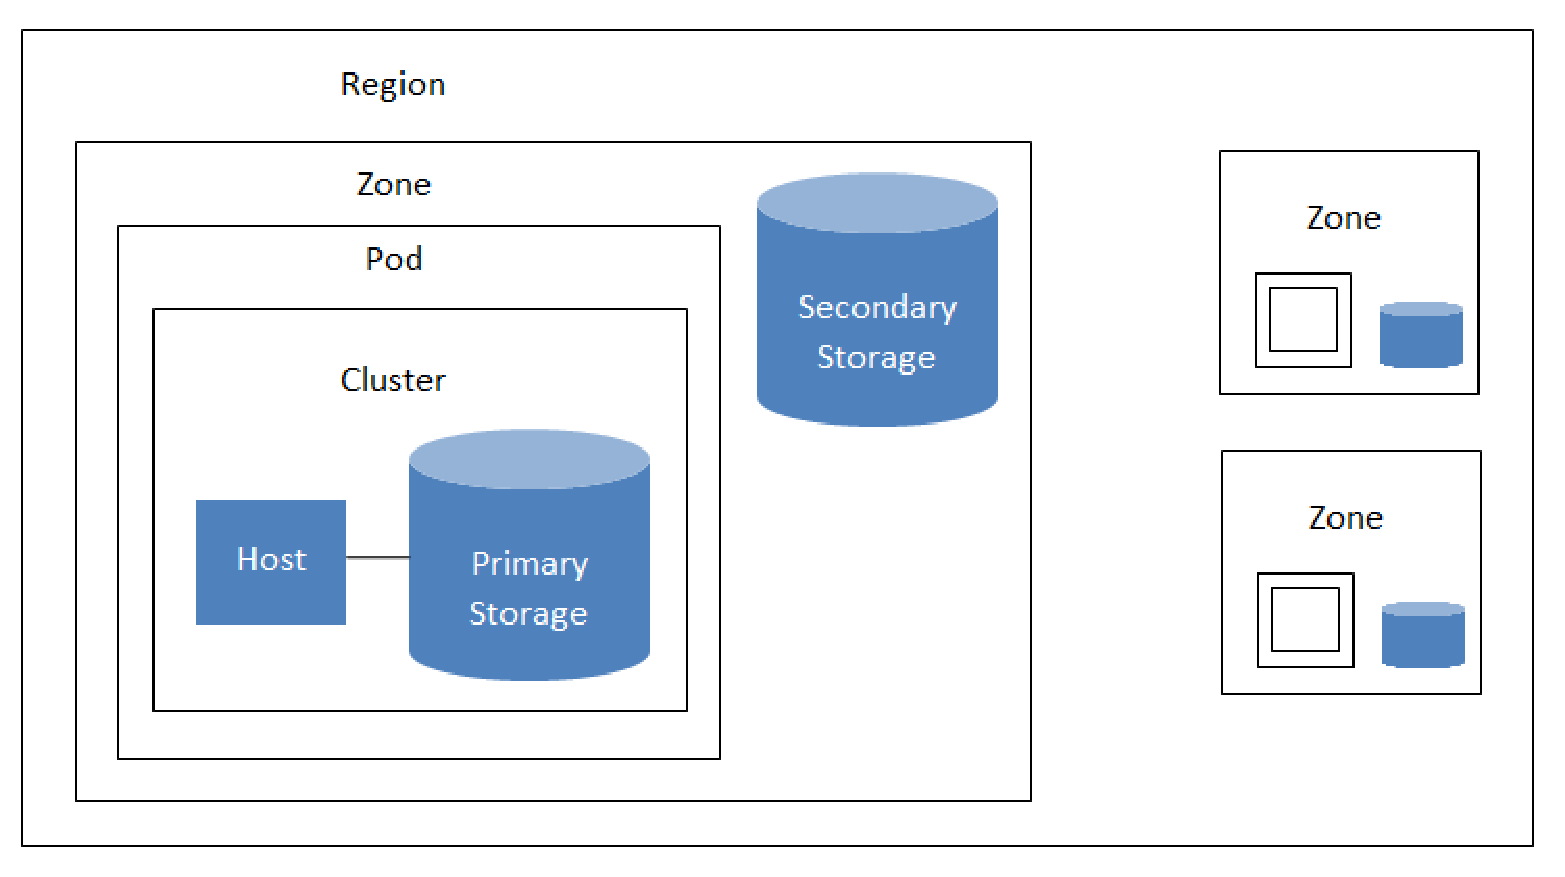
\includegraphics [keepaspectratio=true,scale=0.60]{figuras/cloudstack_structure.eps}
\caption{Visão geral da infraestrutura do Cloudstack}
\cite{cloudstack}.
\label{diagramacloudstack}
\end{figure}

Dessa maneira, afim de se ter um ambiente limpo e com um sistema operacional atualizado, efetuou-se a formtação do disco do servidor \textit{Solarian}, sendo em seguida instalado o sistema operacional \textit{Centos 7}. Assim, com o auxílio da documentação do cloudstack a instalação procedeu sem muitos problemas. Com instalação concluída, já era possível acessar a interface de gerenciamento dando continuidade com as configurações necessárias para criação de máquinas virtuais. Entretanto, a obrigatoriedade de configuração de todos os niveis de abstração, apresentados logo a cima, mostrou-se despendiosa e desnecessária para uma configuração mínima e também para a infraestrutura disponível no LAPPIS. Desse modo, alguns elementos do \textit{cloudstack}, necessários para o ambiente, não apresentaram o comportamento esperado. Um exemplo disso, era problemas recorrentes relacionados com a máquina virtual de sistema, reponsável pelas operações no storage secundário (referenciada por \textit{SSVM}), o que impossibilitava a criação de máquinas virtuais a partir de templates.Em resumo, mesmo com os problemas enfrentados, foi possível a criação de máquinas virtuais nessa plataforma, entretanto a configuração de vários elementos decorrente de sua abstração voltada para uma infraestrutura mais complexa, acabou por tornar difícil o gerenciamento e estabilização do ambiente como um todo, sendo considerado, para o caso em específico do LAPPIS, não sustentável.

O \textit{OpenNebula}, assim como o \textit{cloudstack}, é uma ferramenta de código aberto que emergiu como um projeto de pesquisa em 2005 tendo seu primeiro lançamento público em março de 2008. Oferece uma solução simples mas repleta de funcionalidades para construir e gerenciar nuvens corporativas e \textit{data centers} virtuais. Alem disso, combina tecnologias de virtualização existentes com funcionalides avançadas para fornecimento automático e elasticidade, seguindo uma abordagem \textit{bottom-up}, guiado pelas reais necessidades de adminstradores de sistemas e \textit{devops}\cite{opennebula}.

Em uma configuração mínima  arquitetura do \textit{OpenNebula} é composta por três componentes: \textit{hosts}, \textit{datastores} e \textit{front-end}. O \textit{front-end} é a máquina responsável por disponinbilizar a interface de gerenciamento. Através da rede, monitora os \textit{hosts} e máquinas virtuais, bem como inicia operações relacionadas com máquinas virtuais e \textit{datastores}. Os \textit{hosts} ou \textit{worker nodes} são as máquinas físicas responsáveis pelos recursos físicos essenciais para a criação de máquinas virtuais, é nesta máquina onde o hipervisor será instalado. Por fim, os \textit{datastore} é o \textit{storage} utilizado como repositório de imagens e para manter os discos das máquinas virtuais, em execução. Não precisa ser necessariamente um storage dedicado, podendo ser uma máquina física com mais capacidade de disco ou até mesmo sendo um dos próprios \textit{hosts}.  


\begin{figure}[!htb]
\centering
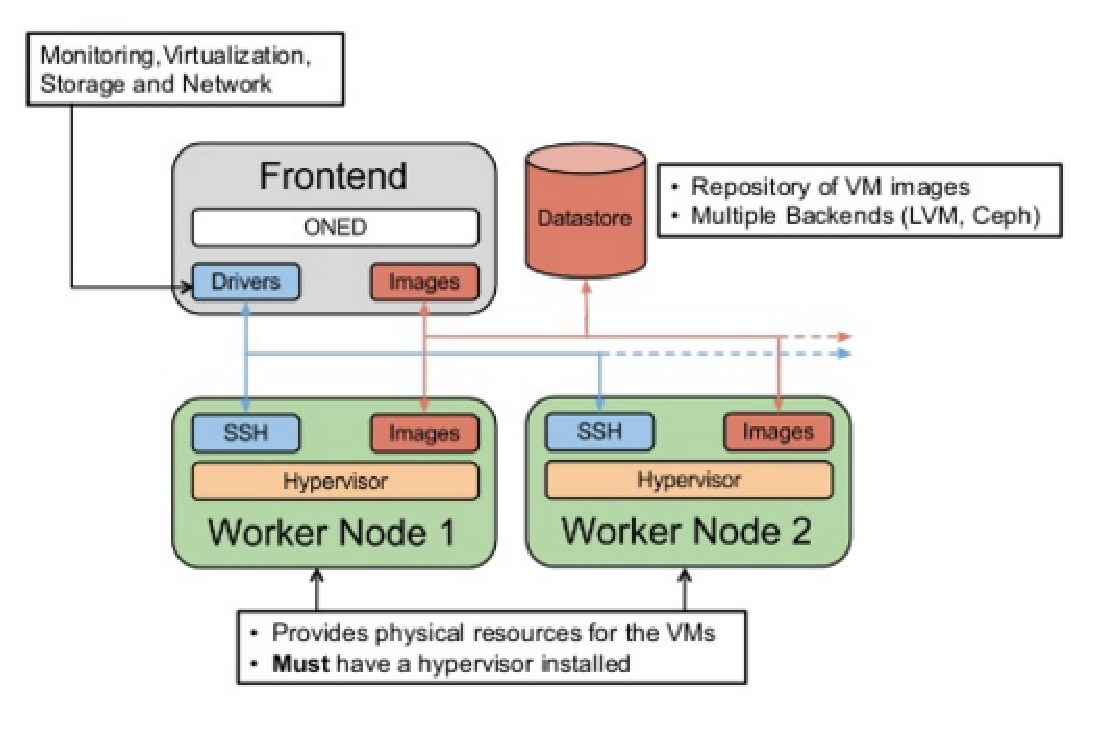
\includegraphics [keepaspectratio=true,scale=0.60]{figuras/opennebula_instalation.eps}
\caption{Visão geral da infraestrutura do OpenNebula}
\cite{opennebula}.
\label{diagramaopennebula}
\end{figure}




O \textit{OpenNebula} possui modelos de implementação tanto para nuvens privadas mais simplifcadas quanto para ambientes de infraestrutura mais complexos. Desse modo, para poucos servidores a implementação do \textit{OpenNebula} é efetuada sem necessidade de ter que se preocupar elementos voltadas para uma infraestrutura maior, que no caso do OpenNebula é chamada de \textit{Federação}. Entretanto, para locais ou empresas que possuem múltiplos \textit{data centers}, que por sua vez, possui vários \textit{clusters} de servidores, o opennebula prover funcionalidades que colaboram para que vários data centers separados regionalmente possam ser gerenciados a partir de uma interface em nuvem com acesso externo. 

Cada instância do opennebula é denominada de zona, desse modo em uma infraestrutura com múltiplas zonas pode ser configuradas como uma Federação. Assim, tem-se um compartilhamento da base de dados entre as zonas(Usuários, grupos). Nessa configuração, uma das zonas tem o papel de \textit{master}, ao qual é o responsável por escrever as informações na base dados, mantendo assim a consistência nos dados\cite{opennebula}.

\begin{figure}[!htb]
\centering
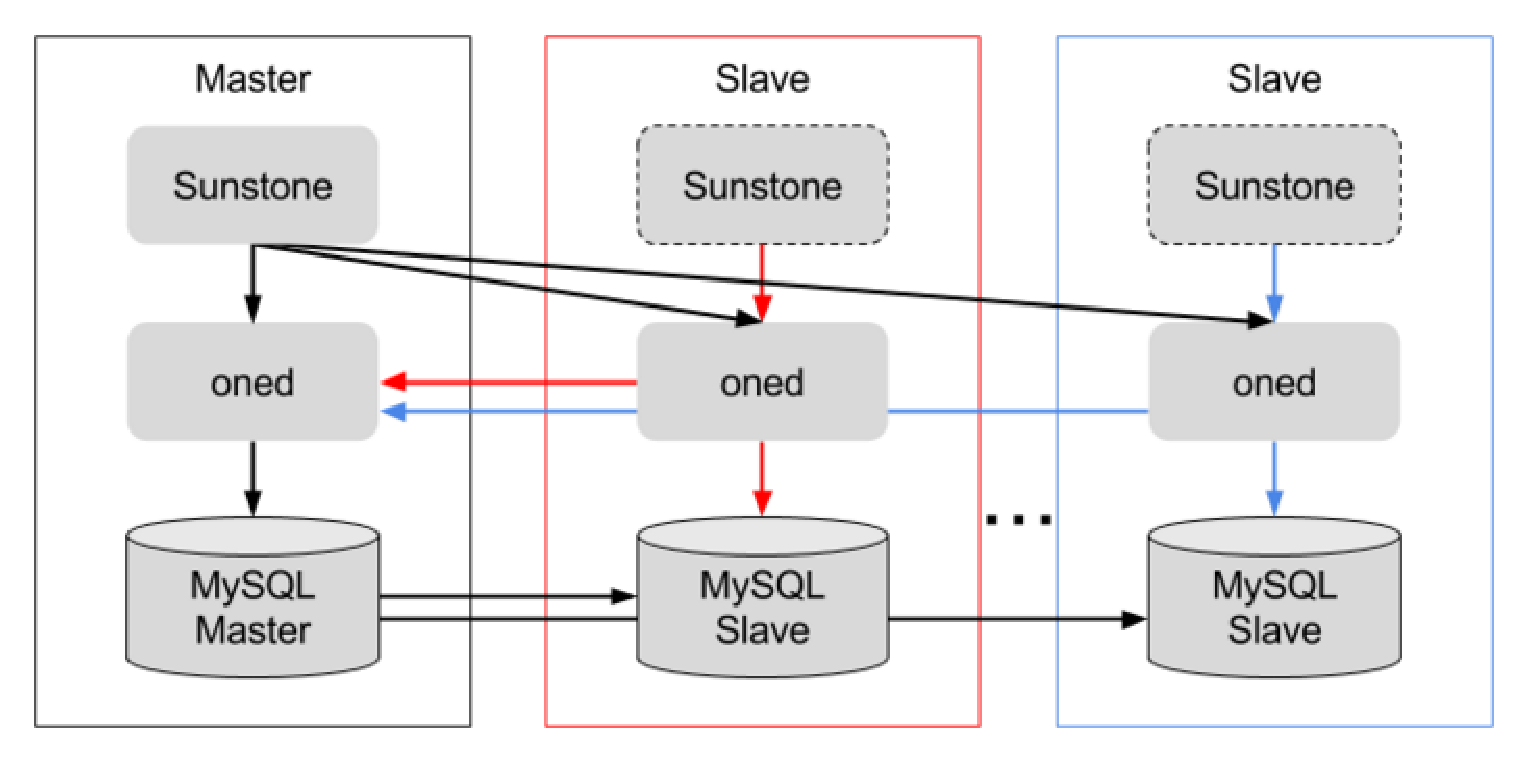
\includegraphics [keepaspectratio=true,scale=0.60]{figuras/opennebula_zone.eps}
\caption{Arquitetura de implantação por zonas}
\cite{opennebula}.
\label{opennebulafederation}
\end{figure}



Para instalação do \textit{OpenNebula}, foram adotados os mesmos procedimentos feitos para testes com o \textit{Cloudstack}: formatação do disco e instalação do sistema operacional \textit{Centos 7}. Dessa forma, destaca-se a clareza e objetividade da documentação do \textit{OpenNebula}, ao qual, apartir da mesma, a instalação prosseguiu sem muitas dificuldades. Para testes iniciais, utilizou-se uma estação convencional de trabalho para ser usada como \textit{front-end} e \textit{datastore}. O servidor \textit{Solarian}, foi então configurado como \textit{worked node}. Após a instalação e as configurações de redes devidamente concluídas no \textit{front-end} e \textit{worked node}, já era possível acessar a interface de gerenciamento. Percebeu-se de início a facilidade e simplicidade tão enaltecidas pela documentação do \textit{OpenNebula}. Assim, sem necessidade de muitas instruções, através da interface de gerenciamento, adicionou-se o servidor \textit{Solarian} como \textit{worked node}. Apartir de então, o \textit{daemon ONED} do \textit{OpenNebula} passou a realizar operações de reconhecimento e monitoramento no servidor \textit{Solarian}, sendo possível a criação de máquinas virtuais sobre o mesmo. Não se teve qualquer tipo de problema ou instabilidade graves na criação de máquinas virtuais, tão logo criadas, ja era possível acessa-las via \textit{ssh}. Destaca-se que a integração da interface de gerenciamento com o \textit{OpenNebula MarketPlace}, possibilitou a disponibilização rápida de máquinas virtuais. O \textit{OpenNebula Marketplace} é um catálogo \textit{online} de imagens pré-configuradas para máquinas virtuais, assim através da sua integração com a interface de gerenciamento já era possível criar máquinas virtuais com sistemas operacionais como \textit{Debian 8} e \textit{Centos 7}, previamente disponibilizados no \textit{OpenNebula Marketplace}. 

Em seguida, afim de se ter uma avaliação inicial de desempenho, tomou-se a decisão de disponibilizar um ambiente de testes para o desenvolvimento do Portal do Software Público (SPB). O SPB é composto de um conjunto de ferramentas com funcionalidades complementares, que são desenvolvidas de forma independentes pelas suas respectivas comunidades\cite{softwarepublico}. Para isso, faz uso de cinco máquinas virtuais, aos quais cada uma possui uma função ou serviço específico. O \textit{deploy} de todo esse ambiente é automatizado, assim com poucos comandos os serviços necessários são instalados em suas respectivas máquinas virtuais. A imagem a seguir apresenta uma arquitetura de implantação do ambiente do Portal do Software Público. 
\begin{figure}[!htb]
\centering
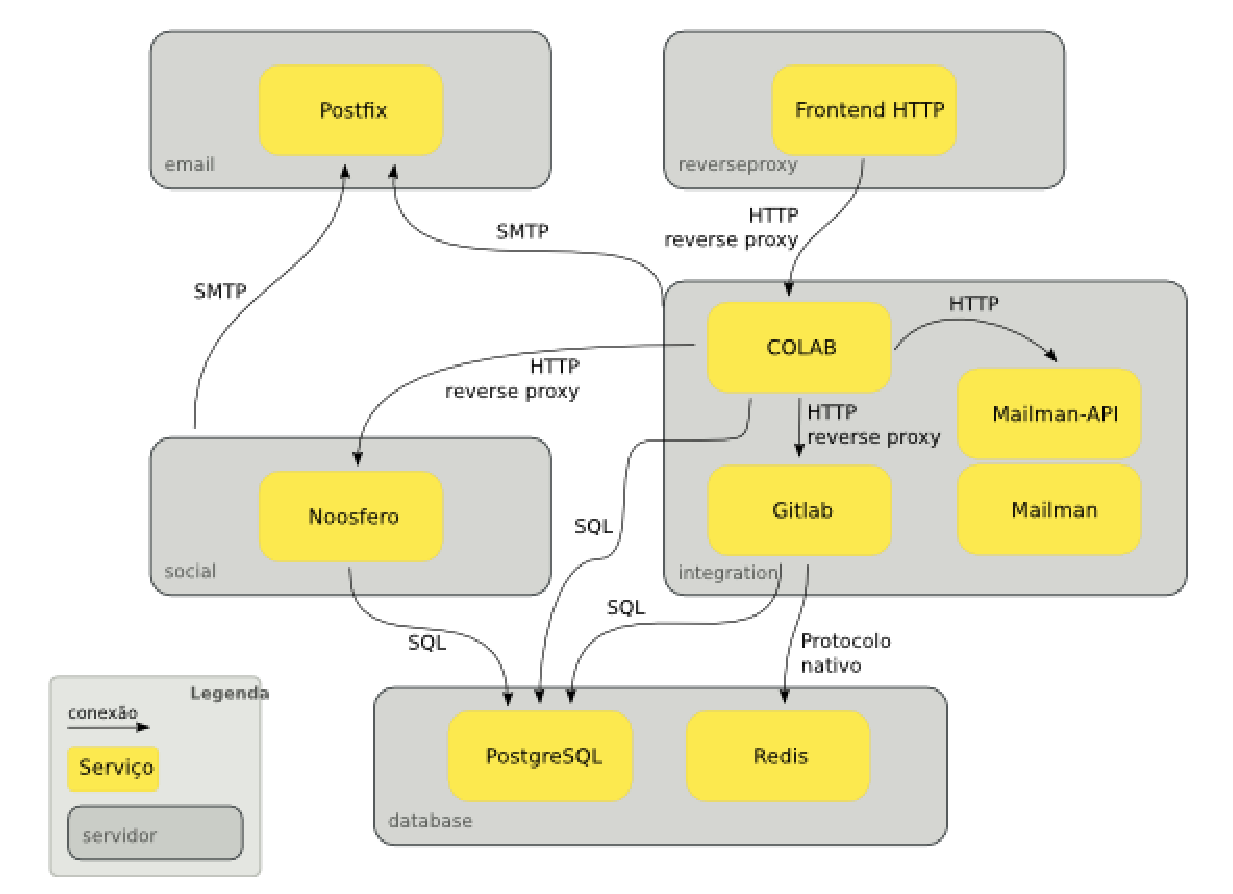
\includegraphics [keepaspectratio=true,scale=0.60]{figuras/arquiteturaSPB.eps}
\caption{Arquitetura do Portal do Software Público}
\cite{softwarepublico}.
\label{SPB}
\end{figure}

Assim, devido a quantidade ferramentas que seriam instalados, só o processo de instalação já seria um ótimo meio de avaliar o desempenho. Portanto, cinco máquinas virtuais foram criadas com o sistema operacional \textit{Centos 7}(necessário para o deploy do SPB), e em seguida, iniciou-se o procedimento de instalação do Portal do software Público nessas máquinas virtuais. Percebeu-se então que havia uma certa lentidão na instalação das ferramentas , e o procedimento que, em condições normais demoraria de 20 a 30 minutos, sob o ambiente virtual récem instanciado havia demorado por volta de 5 horas. Desse modo, alguns possíveis fatores foram listados como possíveis causas dessa lentidão:

\begin{itemize}
\item Uso de uma estação de trabalho de baixo de desempenho como \textit{datastore} e \textit{front-end}.
\item Uso do \textit{System Datastore} na opção \textit{shared}.
\item Imagem de disco no formato \textit{qcow2}
%mysql
\end{itemize}

A estação de trabalho convencional havia sido escolhido apenas para testes iniciais, desse modo, por possuir uma configuração intermediária entre um servidor e estação de trabalho de alto desemepenho, optou-se por utilizar a máquina \textit{Polaris} como \textit{datastore}, \textit{front-end} e também como \textit{worked-node}. Após isso, notou-se uma melhora significativa no tempo de disponibilização de máquinas virtuais mas ainda assim, continuava baixo o desempenho para \textit{deploy} do Portal do Software Público. Então a próxima medida adotada foi a mudança de configuração no tipo de \textit{System Dastore}. O \textit{System Datastore} é uma abstração do OpenNebula ao qual é responsável por manter os discos das máquinas virtuais em execução. Possui três tipos:

\begin{itemize}
\item \textit{\textbf{shared}} - O \textit{System Datastore} é compartilhado entre todos os outros hots usando \textit{NFS}, por exemplo.
\item \textit{\textbf{vmfs}} - Necessário quando o hipervisor utilizado é o \textit{VMware}.
\item \textit{\textbf{ssh}} - Nesse caso, cada host possui seu próprio \textit{System Datastore}.
\end{itemize}

Inicialmente, havia se utilizado como configuração padrão do OpenNebula a opção \textit{shared} para tipo do \textit{System Datastore}. O que se mostrou um equívoco inicial, afinal o \textit{LAPPIS} não possui uma infraestrutura de rede de armazenamento que comporte esse tipo de centralização de armazenamento para máquinas virtuais. Com as operações de escrita em disco das máquinas virtuais tendo que passar através da rede, isso viria a se tornar um grande gargalo. Portanto, a opção adequada nesse caso foi a configuração do \textit{System Datastore} para opçao \textit{ssh}. Teria-se um aumento no tempo na disponibilização de máquinas, entretanto o desempenho melhoraria pois o uso do disco estava local agora. 

Outro fator que impactava no desempenho era o uso de imagens \textit{qcow2}. O \textit{qcow2} é um formato de imagem de disco, ao qual sua vantagem reside no fácil gerenciamento. Afinal, possui suporte para \textit{snapshot}, alocação de espaço no disco é dinâmica e o tamanho de suas imagens é bastante reduzido se comparado com o formato \textit{raw}. Entretanto, possui um baixo desempenho, se comparado ao  próprio \textit{raw}. Uma alternativa incial foi o uso de discos \textit{LVM} para as máquinas virtuais ao invés de imagens de disco como \textit{raw} e \textit{qcow2}, entretanto teve-se problemas com o monitoramento efetuado pelo \textit{ONED}, o que por si só foi um indicativo que para o uso de \textit{LVM} o openenbula ainda não oferece um bom suporte. Então, após investigações sobre o problema de desempenho com imagens de disco no formato \textit{qcow2}, descobriu-se que os problemas de desempenho com essas imagens podem ser minimizados utilizando opções de \textit{cache} em disco. Dentre as opções disponibilizadas pelo \textit{OpenNebula} (\textit{writeback, writethrough, directsync, unsafe} a que mostrou mais efetiva em termos de desempenho e segurança foi a opção \textit{writeback}.

Após esses procedimentos, notou-se um aumento considerável no desempenho de escrita de disco nas máquinas virtuais, de modo que as aplicações passaram a serem instaladas sem qualquer problema relacionado com desempenho, possibilitando assim que o \textit{deploy}  Portal do Software Público para ambiente de testes pudesse ser feito sem grandes problemas. Com isso, emfim tinha-se finalmente chegado a um ponto de estabilização da infraestrutura como um todo, os próximos passos englobariam então a disponibilização dos serviço providos pelo LAPPIS sob a nova plataforma em nuvem, bem como utilização do servidor \textit{Imperius} sob essa plataforma.  

\section{Consolidação da Infraestrutura}
Após os testes iniciais e a disponibilização de alguns serviços, tinha-se uma infraestrutura estável e pronta para ser utilizada como provedora de serviços. Como etapa final, então era necessário incorporar o servidor \textit{Imperius} sob a plataforma em nuvem. Antes disso, fazia-se necessário replicar os serviços, que atualmente estavam em execução no servidor \textit{Imperius}. Após te-lo feito, o servidor \textit{imperius} fora incorporado sob a nova plataforma consolidando assim toda a infraestrutura física de servidores sob a nova plataforma em nuvem. A Figura \ref{fig:opennebula_lappis} apresenta o modelo de implantação final do \textit{OpenNebula}.

\begin{figure}[!h]
\centering
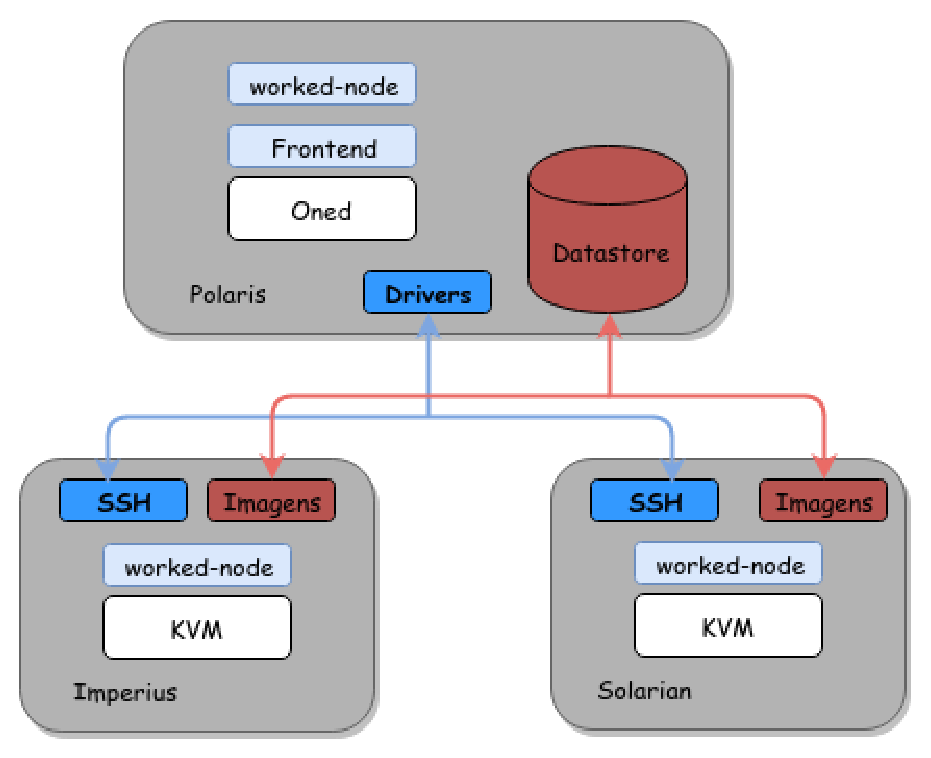
\includegraphics [keepaspectratio=true,scale=0.53]{figuras/cloud_implation.eps}
\caption{Implantação do \textit{OpenNebula}}
\label{fig:opennebula_lappis}
\end{figure}


Serviços como \textit{Redmine}, \textit{Dotproject} se mantiveram, a \textit{Services} que antes era utilizado tanto como \textit{Firewall} como máquina para acesso externo, fora configurada apenas como máquina de acesso externo. Uma outra máquina virtual para \textit{Firewall} fora criada, sendo nela colocados os ip's públicos. Outros serviços foram disponibilizados, a Figura \ref{fig:vm_infra} apresenta um visão geral de todos eles. A seguir é feita uma breve descrição dos principais serviços recém disponibilizados:

\begin{itemize}
\item \textbf{\textit{Proxy}}: Utilizada como um \textit{proxy} de cache, promovendo assim um melhor desempenho na transferência de pacotes que já foram baixados.
\item \textbf{\textit{Boca}}: Máquina virtual utilizada para disponibilização do \textit{BOCA}, servindo dessa forma como \textit{juiz online} para competições de programação para disciplina de \textit{Tópicos Especiais em Programação}.
\item \textbf{\textit{Moodle}}: Responsável pela disponibilização do \textit{Moodle} para disciplinas de Computação Básica.
\item \textbf{\textit{Mirror}}: Reponsável por servir de \textit{espelho} de alguns repositórios utilizados pelo Portal do Software Público.
\item \textbf{\textit{PortalFGA-Homologação:}} Ambiente de homologação do Portal da FGA.

\end{itemize}


\begin{figure}[!h]
\centering
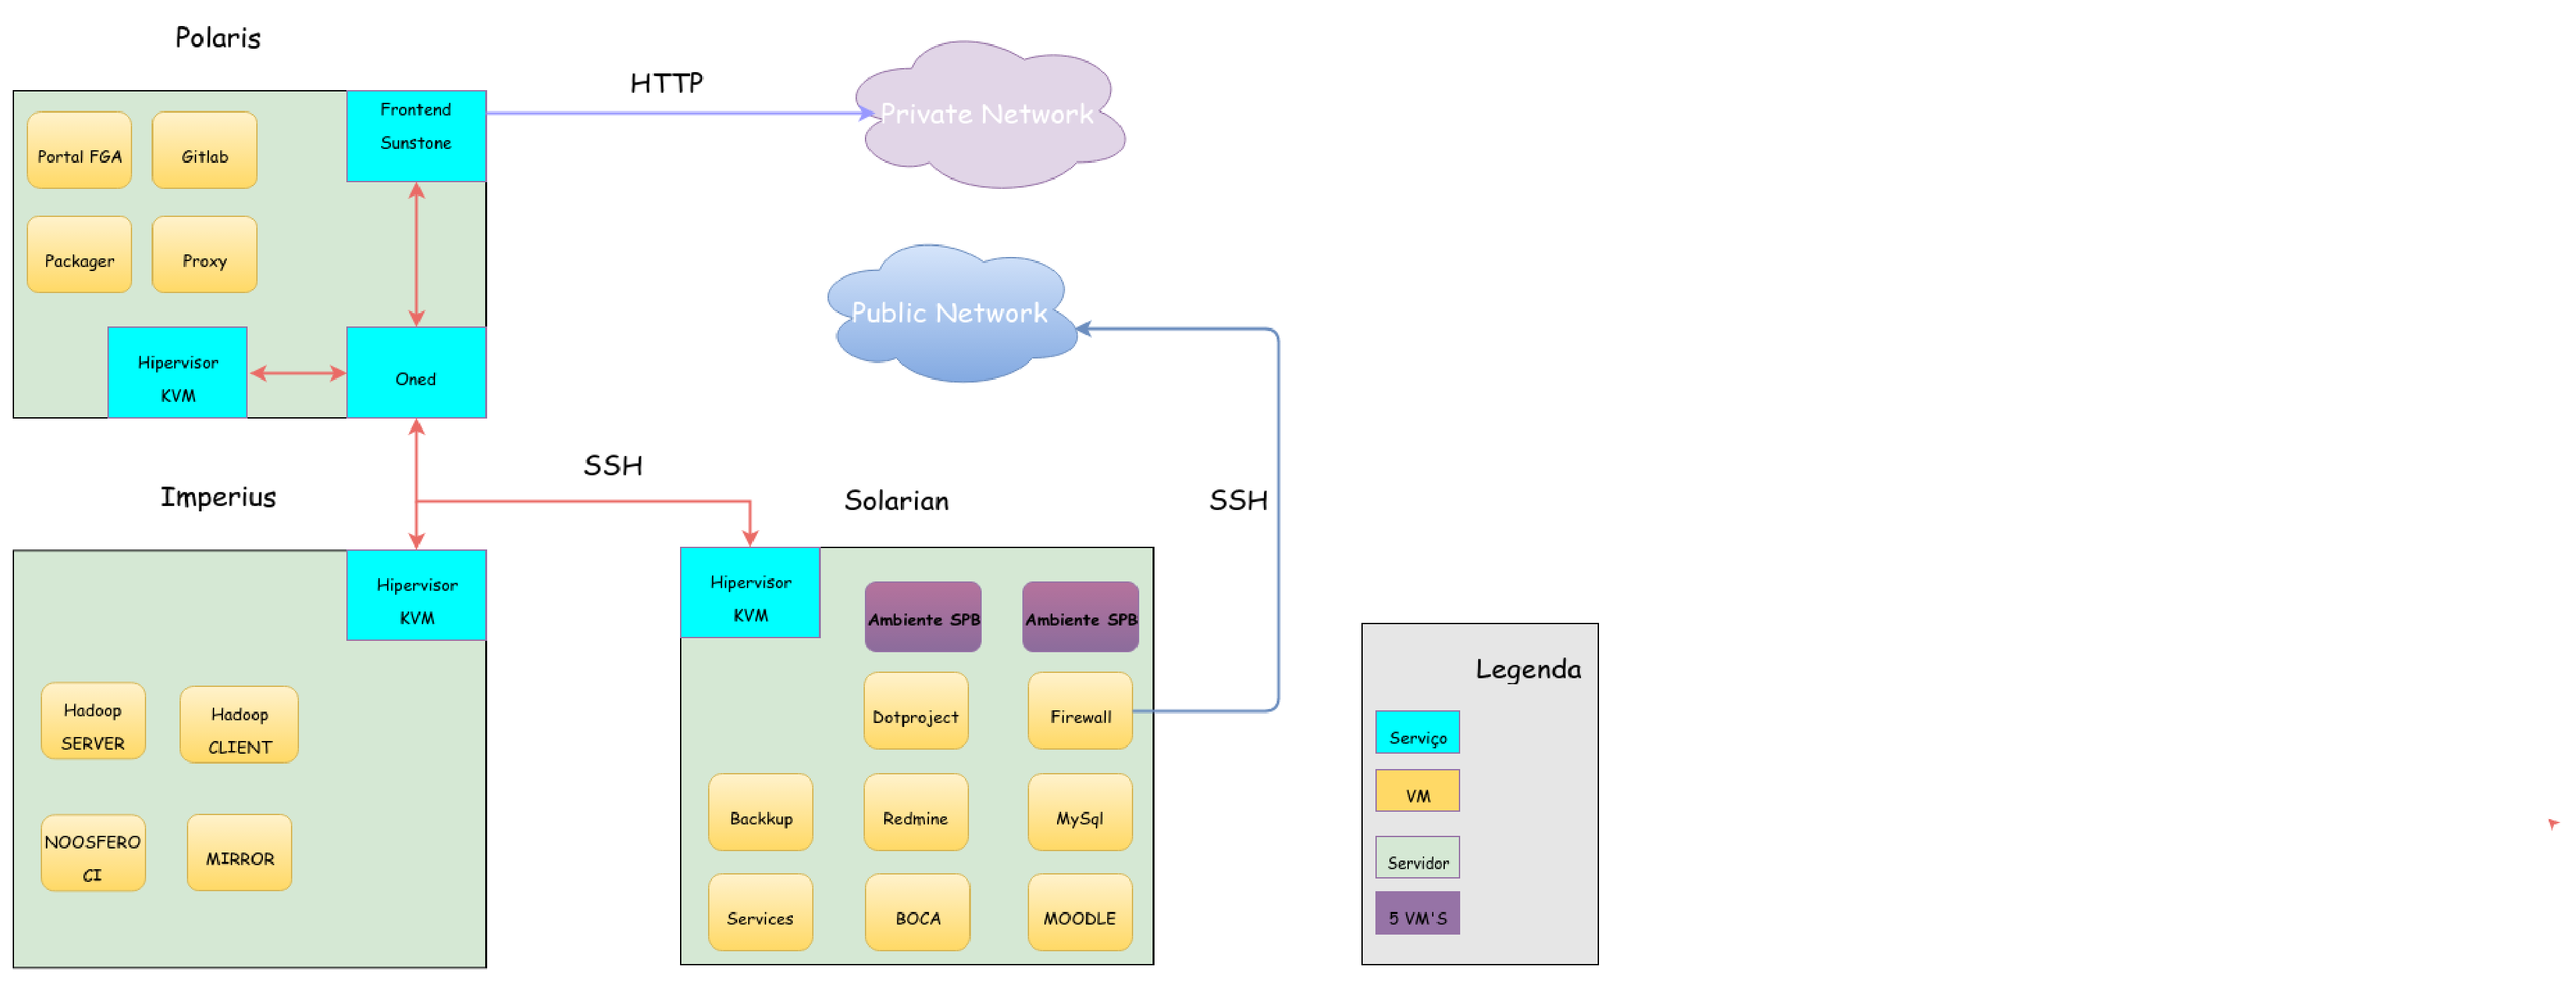
\includegraphics [keepaspectratio=true,scale=0.4]{figuras/vm_infra.eps}
\caption{Visão geral da Infraestrutura}
\label{fig:vm_infra}
\end{figure}

Outro procedimento adotado foi o uso da ferramenta \textit{Chef} em conjunto com o \textit{Chake} para automatização, tanto no provimento da plataforma em nuvem, quanto na disponibilização de serviços. O \textit{Chef} é um \textit{Framework} que tem como objetivo transformar uma complexa infraestrutura em código,  tornando mais fácil a disponiblização de aplicações em qualquer ambiente seja ele físico ou virtual \cite{chef}. É composto pelo \textit{Chef Client} e pelo \textit{Chef Server}, sendo que o \textit{chef client} é responsável por efetuar as configurações necessárias na máquina pretendida a partir de informações localizadas e gerenciadas pelo \textit{chef server} .Um meio de se utilizar o \textit{Chef client} sem ter que o usar o \textit{Chef Server} é usar a versão código aberto do \textit{Chef client}, o \textit{Chef Solo}. 

O \textit{chake} é uma ferramenta que ajuda a gerenciar múltiplos ambientes sem a necessidade de se utilizar o \textit{chef server}. As configurações são geralmente implantadas via \textit{rsync} com o auxílio do \textit{SSH}, e aplicadas invocando o \textit{chef solo} em cada ambiente. O uso dessas ferramentas contribui para gerencia do serviços oferecidos, promovendo também um meio de compartilhamento de conhecimento através do código. Com isso, como uma iniciativa inicial para automatização bem como documentação da infraestrutura, desenvolveu-se neste trabalho arquivos de configurações, utilizando o \textit{Chake} e \textit{chef solo}, para alguns serviços disponibilizados: \textit{Dotproject}, \textit{Redmine}, \textit{OpenNebula Front end}, \textit{OpenNebula Worked Node}.










%TO DO adequar e estrutura o trecho a seguir
%Assim como feito no caso do cloudstack , foi feita uma limpeza no servidor \textbf{Solarian}, afim de se ter um ambiente limpo, e novamente utilizou-se o \textit{O centos 7}.Assim como no cloudstack, um dos pontos fortes do opennebula foi sua documentação clara e objetiva com relação a instalação. Dessa maneira a instalação prosseguiu sem muitos problemas.Para testes iniciais , utilizou-se uma máquina de estação convencional para atuar como \textit{front-end} e como storage. O servidor \textit{Solarian} ficou como \textit{hosts}.Com as configurações de redes e instalação terminada, já era possível acessar a interface de gerenciamento. Logo de iniciou-se era notória a facilidade e simplicidade/ , tão enaltecida pela documentação do \textit{OpenNebula}. Através da interface de gerenciamento, adicionou-se o servidor \textit{Solarian} como \textit{host}, e em seguida, fora feita a configuração de rede virtual deixando-a sob o mesmo \textit{gateway} ao qual o servidor \textit{Solarian} e o \textit{front-end} estava conectado. Dessa forma prosseguiu-se com a criação de máquinas virtuais sem muitas dificuldades e sem qualquer problemas graves de instabilidades. Dessa forma, como forma de testar o estabilidade e desempenho do ambiente na disponibilização dos serviços, um dos primeiros passos foi a instanciação do ambiente do portal do software público. Em resumo, tal ambiente é constituído por cinco máquinas virtuais , aos quais possui diversas aplicações em cada uma delas sendo  que alguma delas comunicam entre si. O deploy desse ambiente é automatizado, assim com poucos comandos inicia-se a instalação automática das aplicações que compõem o Portal do software Público através das cinco máquinas virtuais. Desse modo, utilizou-se tal procedimento como um meio inicial de avaliar o desempenho do ambiente como todo. A imagem a seguir apresenta a estrutura do portal do software público. 


%código aberto que tem como foco trazer siplicidade na disponibilização de plataformas em nuvems hibridas e privadas.

%O cloudstack se mostrou de fácil instalação, usando no servidor físico um sistema operacional \textit{Centos 7}. Tão logo concluído, a interface de gerenciamento já se encontrava disponivel. O restante da configuração \textit{Ip's}, \textit{storage}, \textit{host}(servidor físico), deve ser feita via interface. E foi aí que encontrou-se dificuldade: A obrigatoriedade de configuração seus niveis de abstração mostrou-se bastante despendiosa para uma configuração mínima.Muitos elementos separados que quando se integram junto pode não se comportar da forma esperada.Outro fator que dificultou bastante na configuração foi suas \textit{VM's} criadas automaticamente.De maneira geral, foi possível a criação de máquinas virtuais, entretanto todo o ambiente demonstrou-se bastante instável, tendo assim bastante dificuldade na disponibilização de ambientes virtuais iniciais para testes.  

